\chapter{Implementation}

The implementation section below will explain what technologies were used and how they were implemented into ChatX.

\section{Code Standards}
Since this project makes use of two different programming languages it would be unwise to not set a code standard. So a code standard was set for each programming language.

\subsection{Java}
Class names must start with a capital letter.
Variables must start with lowercase letters, private ones should be refereed by using ".this".
Curly brackets are to be in their own lines at all times.
Method names must start with a lowercase letter.


\subsection{C\#}
Class names must start a capital letter.
Variables must start with lowercase letters, private ones should be refereed by using ".this".
Curly brackets are to be in their own lines at all times.
Method names must start with a capital letter.

\section{Client}

\subsection{Java Client}

The java client has been written as the first client and will be used as the test client as it is possible to have a console application.

\section{Cryptography}

To make the communication secure the clients implements an RSA encryption to encrypt all messages sent. RSA is a Public- Private key (asymmetric) encryption algorithm. RSA encryption is a standard for encrypting and is practically impossible to decode due to prime factorization. The general idea is that it is easy to find the product of two large primes, but it is hard to factor a large product and find the primes.

RSA was originally made by Ronald Linn Rivest along with Adi Shamir and Len Adlemanand published in their paper A Method for Obtaining Digital Signatures and Public-Key Cryptosystems\cite{RSA}.

To be able to apply RSA encryption, 6 variables are needed; $d$, $e$, $n$, $p$, $q$ and $\varphi$(phi). $d$, $p$, $q$ and $\varphi$(phi) should be kept secret at all time to keep this encryption secure. Let $p$ and $q$ be a prime number, lets for simplicity say $p=7$ and $q=13$. In practice these 2 numbers would be larger depending on the numbers of bits used for encryption. $n$ is defined as in equation \ref{RSA:n}.

\begin{equation}
n = p \times q
\label{RSA:n}
\end{equation}

In this case $n=91$. Additional $n$ have the bit-length dependent on security of the encryption. If the encryption should be 1024 bit, when $n$ would be a 1024 bit number. $\varphi$ or $\varphi(n)$ is found by using equation \ref{RSA:phi}.

\begin{equation}
\varphi = (p-1)(q-1)
\label{RSA:phi}
\end{equation}

For this example $\varphi = 72$ and it is now possible to find $e$ which is the public exponent. $e$ is a random prime and have two requirements which must be met; $e$ must be a relative prime of $\varphi$, ie. $e$ and $\varphi$ have no common factors and $e$ must be an integer such that $1 < e < \varphi$. For this example let $e=7$. The public key is now available as $n$ and $e$ is known and can be given out.

Lastly we calculate $d$ which is the private exponent using extended euclidean algorithm. Equation \ref{RSA:d} is used for finding $d$.

%https://www.youtube.com/watch?v=moqmFy39Itc
\begin{equation}
d = e^{-1} \textrm{ mod } \varphi
\label{RSA:d}
\end{equation}

From equation \ref{RSA:d} $d=31$ and it is possible to further check if this is correct by using equation \ref{RSA:check} which in this case it is, and the private key is now defined by $n$ and $d$.

\begin{equation}
e \times d \textrm{ mod } n = 1
\label{RSA:check}
\end{equation}

Now where both the public and private keys are assigned, they can be used to encrypt and decrypt messages. If the message "Hi" were to be decrypted it would first need to be translated into a number, eg. as 8 and 9. It is now possible to encrypt both letter individually by using equation \ref{RSA:Encrypt} which gives the output cipher text $C$, and as well as decrypt it again with equation \ref{RSA:Decrypt}.

\begin{equation}
C=M^e \textrm{ mod } n \quad \textrm{Where M $<$ n}
\label{RSA:Encrypt}
\end{equation}

\begin{equation}
M=C^d \textrm{ mod } n
\label{RSA:Decrypt}
\end{equation}

In the computer world when encrypting data, a padding is often used. Padding is often used to fill out byte blocks. For instance, if the message "Hi!" would had the byte block [48 69 21]. This block size is only of 3 bytes, but the encryption algorithm might read a block of 8 at a time which would mean the block needs 5 more bytes. There is multiple way of padding a message, such as zero-padding [48 69 21 00 00 00 00 00], padding with the same value as the number of bytes [48 69 21 05 05 05 05 05]\cite{PADDING}. When the padding is done a block can be sent to the encryption algorithm to produce the cipher text.

\section{Server}

The server is the part of the system that handles the users and which rooms they are in. The server is split up with the three layer architecture. Model, Controller and GUI. 

The Model layer consists of four classes, User, Room, Message and Lobby. User class is used to handle the users in the system. The Room class keeps track of which users are in which rooms and allows them to send messages between them in the rooms. The Message class is what users use to send chat messages with. The lobby class works almost the same as the room class, it's a room class that will never be deleted and where all users are put in when they log in.


The server has a Interface which contains the necessary methods to implement any Messaging Queue system if RabbitMQ should ever be replaced, for now RabbitMQ is the messaging queue system that listens to commands from the service and depending on what the service requests from the server, sends messages back to the service.

The Controller is where the servers logic has been implemented. It has one class: ServerController. It keeps track of how many users are online in the system, which rooms those users are in, how many rooms there are and also which usernames are already taken. ServerController uses the singleton pattern, meaning there can only be one instance of ServiceController on the server. This has been done because otherwise it would be difficult to handle which users and rooms belong to which instances. Service Controller has a event handler that checks what commands it recieves from Service, the event handler looks into what command the message has and sends it to the appropriate method. ServerController consists of seven methods, JoinRoom, SendMessage, RequestRooms, LoginRequest, VerifyAndLockUsername, and ReleaseUsername. Whenever a user logs in a socket connection is created between the Server and the users in their rooms, which allows them to chat with eachother. Lastly ServerController makes use of the same Config file used in the Service. It helps showing how the messages from RabbitMQ should be understood for both sides.



The GUI for the server is to control the server. It can turn on the Server so it starts listening on any incoming messages from the Service, and it can be turned off. 


\section{Webservice}
The webservice written in C\#, and is implemented using Windows Communication Foundation (WCF). 

The function of webservice is to be a broker between the client and the server(s); whenever a client interacts with the system, be it sending a message or requesting a list of rooms, it needs to go through this service. The service will then  contact the server(s) through a queue system, currently RabbitMQ, through which the servers also sends their response. The communication can be seen in figure \ref{fig:Communicationdiagram}.

The service consists of:
\begin{itemize}
 \item The exposed functionality available to the clients. This is done through the usual way with an interface as the service contract, and an implementation.

 \item A server distributor. The idea of this is to handle what servers are available, what their IP's are and what port-numbers the socket-connections should be created to go to. 
 
 \item A message queue driver. This handles all functionality related to the messaging queue system.
 
 \item A config class file. This file statically contains the formats of the actual messages send and received through the messaging queue system.

\end{itemize}

The first three of the above items all inherits from the interfaces IChatXService, IServerDistributor and IMQDriver respectively. The first interface is implemented, as this is common, good practice for services. The next two has interfaces to make it easier to replace the actual implementations at a later state of development and even deployment. At the moment, the implementation of the server distributor only distributes to one server, and the only messaging system implementation uses RabbitMQ. But since the implementations are coded against an interface, the only change needed to switch to another implementation is at the initialization of the object.
Below, in figure \ref{fig:ServiceArchitecture}, the service is illustrated:

\begin{figure}[h]
	\centering
	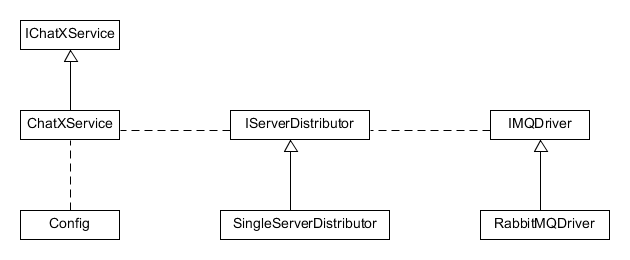
\includegraphics[width=0.7\linewidth]{img/ServiceArchitecture}
	\caption[Communication-diagram]{ChatX Service Architecture}
	\label{fig:ServiceArchitecture}
\end{figure}

The lines between ChatXService, IServerDistributor and IMQDriver are dotted to illustrate the statelessness of the service.

\section{RabbitMQ}